\appendix
\chapter*{附录}
\section*{github commit记录}
\begin{figure}[htbp]
    \centering
    
\includegraphics[width=0.8\textwidth]{github1.png}
    \caption{github1}\label{fig:github1}
    \vspace{\baselineskip}
    \end{figure}
    \begin{figure}[htbp]
        \centering
        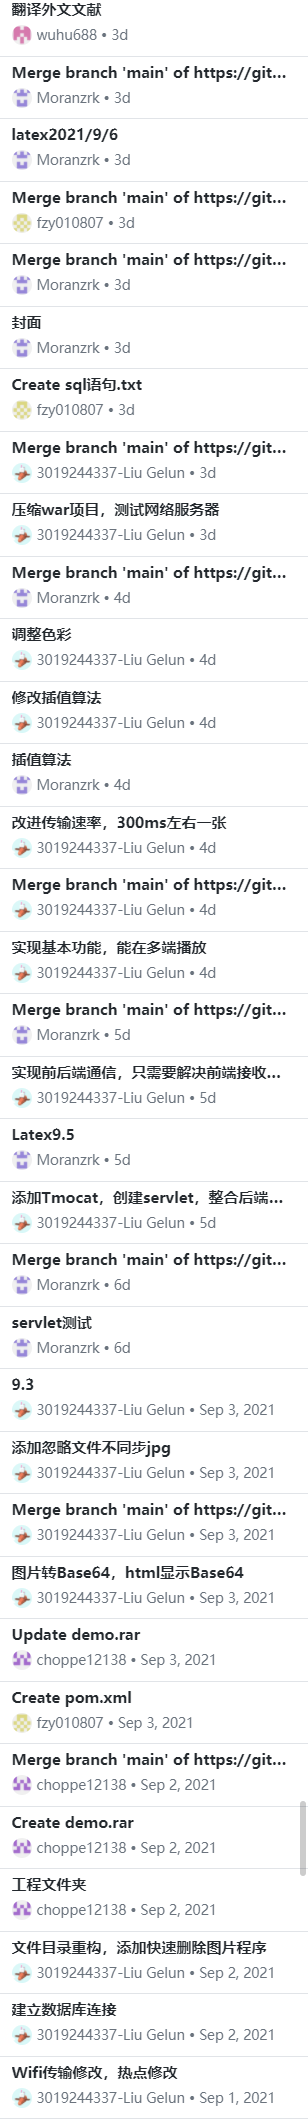
\includegraphics[width=0.8\textwidth]{github2.png}
        \caption{github2}\label{fig:github2}
        \vspace{\baselineskip}
        \end{figure} 
        \begin{figure}[htbp]
            \centering
            
\includegraphics[width=0.8\textwidth]{github3.png}
            \caption{github3}\label{fig:github3}
            \vspace{\baselineskip}
            \end{figure}
            \begin{figure}[htbp]
                \centering
                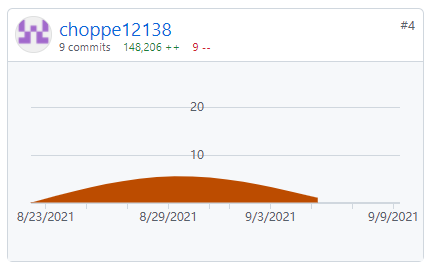
\includegraphics[width=0.8\textwidth]{github4.png}
                \caption{github4}\label{fig:github4}
                \vspace{\baselineskip}
                \end{figure}
    \clearpage
\section*{异构计算的uid及截图}

\begin{figure}[htbp]
\centering
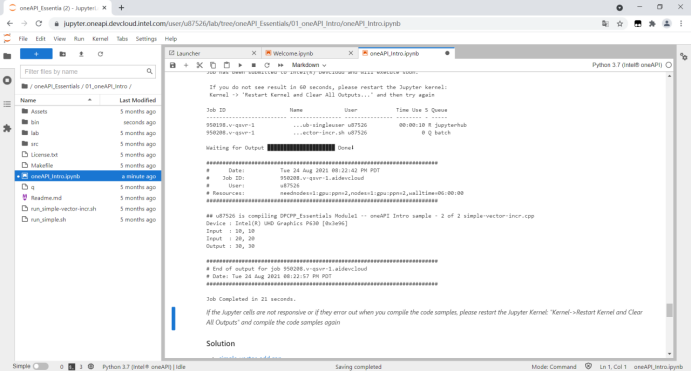
\includegraphics[width=0.8\textwidth]{zrk.png}
\caption{郑睿恺截图uid=u87526}\label{fig:zrk}
\vspace{\baselineskip}
\end{figure}
\begin{figure}[h]
\centering
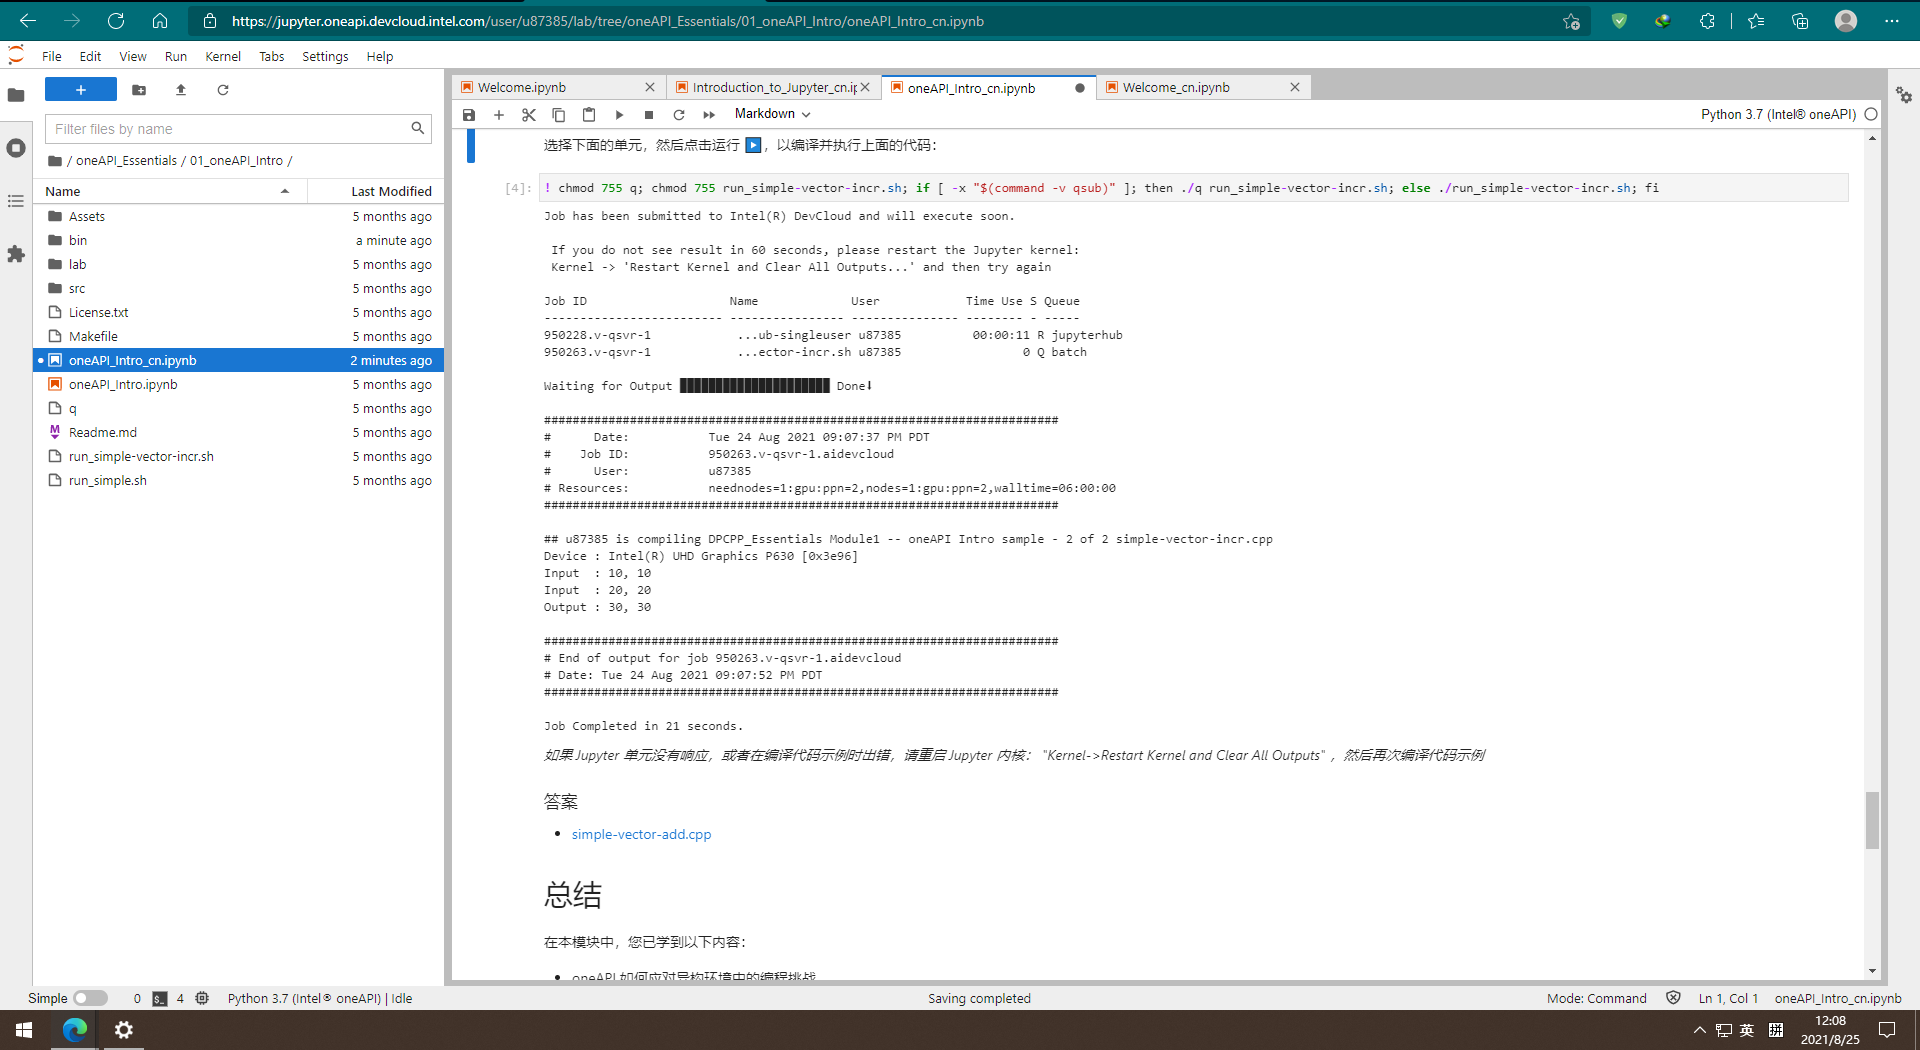
\includegraphics[width=0.8\textwidth]{lgl.png}
\caption{刘格伦截图uid=u87385}\label{fig:lgl}
\vspace{\baselineskip}
\end{figure}
\begin{figure}[h]
\centering
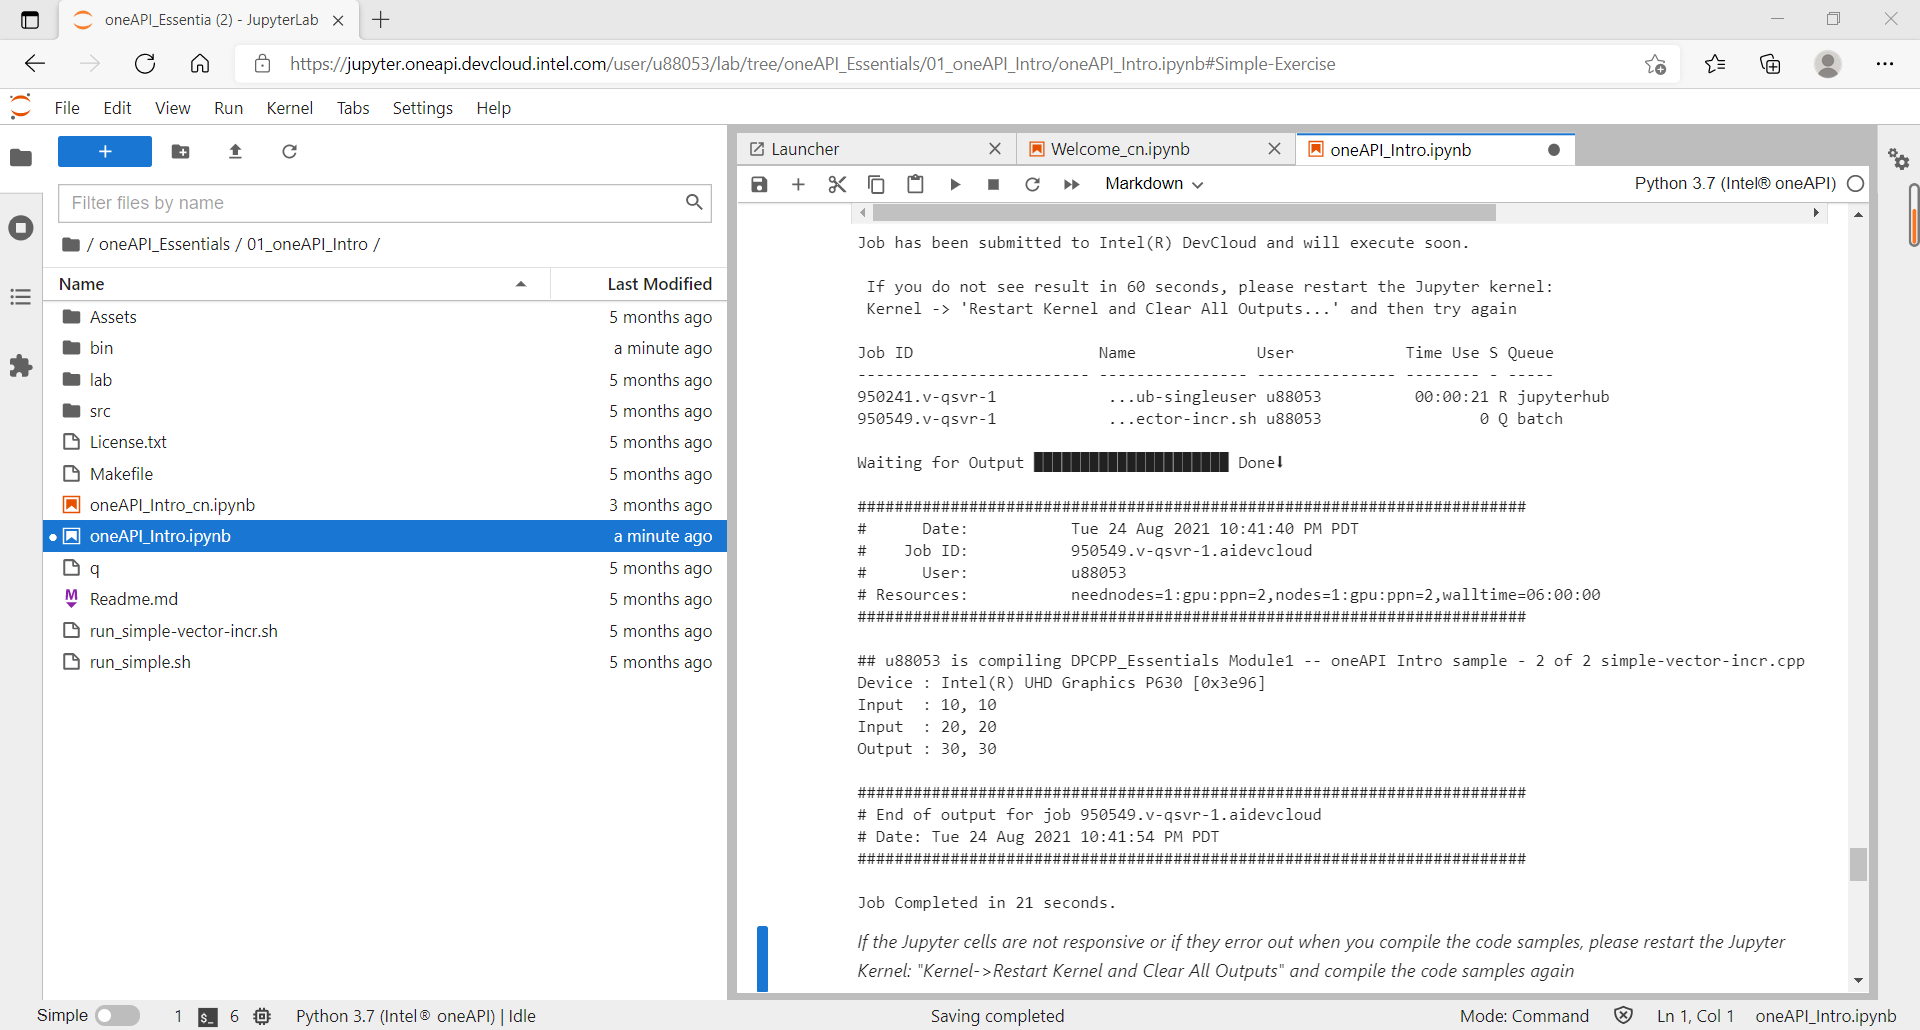
\includegraphics[width=0.8\textwidth]{fzy.png}
\caption{樊振宇截图uid=u88053}\label{fig:fzy}
\vspace{\baselineskip}
\end{figure}    
\begin{figure}[h]
\centering
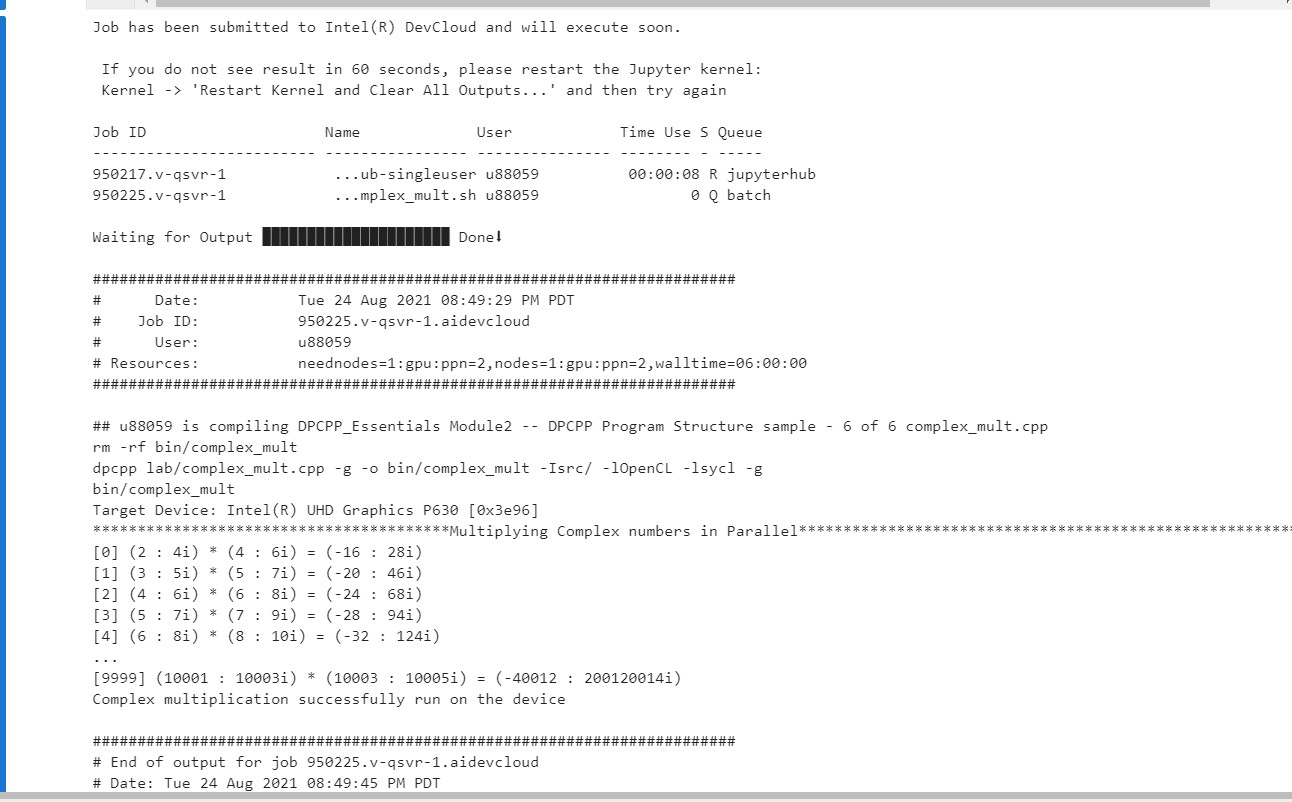
\includegraphics[width=0.8\textwidth]{lsj.jpg}
\caption{李世军截图uid=u88059}\label{fig:lsj}
\vspace{\baselineskip}
\end{figure}
\begin{figure}[h]
\centering
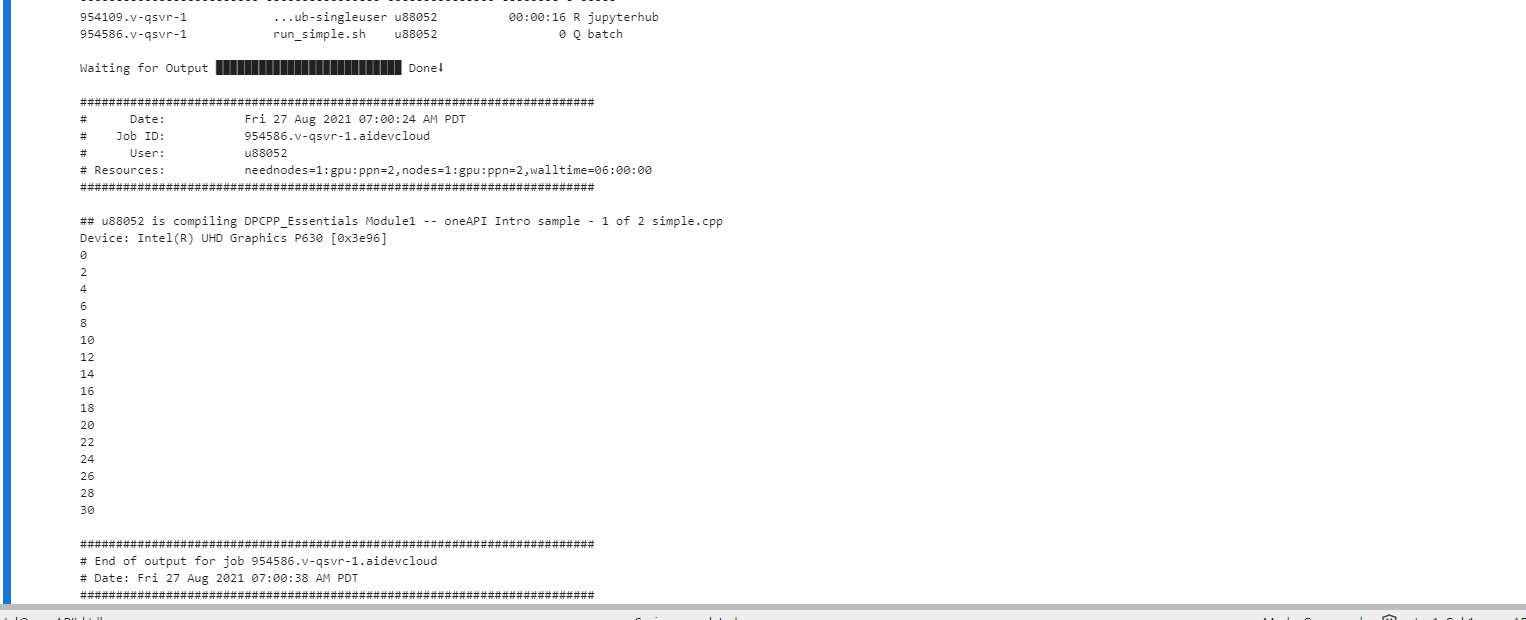
\includegraphics[width=0.8\textwidth]{zzh.png}
\caption{周子涵截图uid=88052}\label{fig:zzh}
\vspace{\baselineskip}
\end{figure}
\clearpage
\section*{参考文献}
[1]陈诚,何锦清,孙华.基于MLX90640探头的热成像图划分区域的研究[J].电子制作,2021(05):88-90+76.

[2]翟靖宇,陈金立,乔欢.基于MLX90640和STM32的人体红外热成像仪[J].电子测试,2021(15):12-14+20.

[3]MLX90640Driver

[4]MLX90640 Thermal Camera 用户手册



